% !TEX root =  ../unref_general.tex

\section{Data Structures}
\label{sec:DataStruct}
This section details the partition of the computational domain in a finite element mesh. In particular, we briefly define the genealogy tree properties and mesh operations for a given element (\cref{subsec:GenTree,subsec:SuppRef}). In \cref{subsec:Removable} we define the concept of removable basis functions. For further details, see Darrigrand et al. \cite{darrigrand2020painless}.

\subsection{Genealogical tree}
\label{subsec:GenTree}
Following \cite{zander2015multi,zander2016multi,zander2017multi}, we define the genealogy tree properties for a given arbitrary element $K$. \Cref{fig:Hierarchi2D,fig:Hierarchi3D} show hierarchical isotropic mesh element subdivision for $2$D and $3$D cases. We restrict ourselves to quadrilateral/hexahedral elements.

\begin{figure}
  \begin{subfigure}[]{0.45\textwidth}
    \begin{center}
      \centering
      \begin{tikzpicture}[scale = 1]
        \draw[xstep=1, ystep=1, black] (0,0) rectangle (3,3);
      \end{tikzpicture}
      \caption{Unrefined $2$D element}
      \label{subfig:unref2Delement}
    \end{center}
  \end{subfigure}
  \begin{subfigure}[]{0.45\textwidth}
    \begin{center}
      \centering
      \begin{tikzpicture}[scale = 1]
        \draw[xstep=1, ystep=1, black] (0,0) rectangle (3,3);
        \draw[xstep=1.5, ystep=1.5, black] (0,0) grid (3,3);
      \end{tikzpicture}
      \caption{Refined $2$D element}
      \label{subfig:ref2Delement}
    \end{center}
  \end{subfigure}
  \caption{Hierarchical isotropic mesh element subdivision for $2$D cases.}
  \label{fig:Hierarchi2D}
\end{figure}

\begin{figure}
  \begin{subfigure}[]{0.45\textwidth}
    \begin{center}
      \centering
      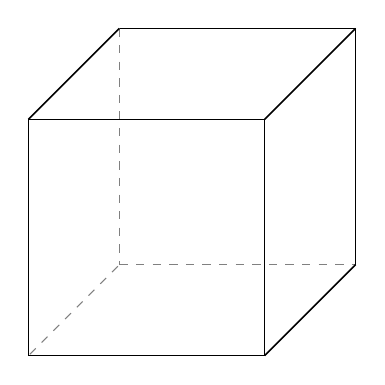
\begin{tikzpicture}[scale = 1]
        %%%%%%%%%%%%%%%%%%%%%%%% Cara trasera %%%%%%%%%%%%%%%%%%%%%%%%%%%%%%%%%%%
        \draw[gray, fill opacity=0.5, dashed] (0,0,0) -- (3,0,0); %Edge inferior punteado
        \draw[line width=0.2mm] (3,0,0) -- (3,3,0); %Edge derecho
        \draw[line width=0.2mm] (3,3,0) -- (0,3,0); %Edge superior
        \draw[gray, fill opacity=0.5, dashed] (0,3,0) -- (0,0,0); %Edge izquierdo punteado
        %%%%%%%%%%%%%%%%%%%%%%%% Cara delantera %%%%%%%%%%%%%%%%%%%%%%%%%%%%%%%%%%
        \draw[line width=0.2mm] (0,0,3) -- (3,0,3); %Edge bajo
        \draw[line width=0.2mm] (3,0,3) -- (3,3,3);
        \draw[line width=0.2mm] (3,3,3) -- (0,3,3);
        \draw[line width=0.2mm] (0,3,3) -- (0,0,3);
        \draw[line width=0.2mm] (0,3,0) -- (0,3,3);
        \draw[line width=0.2mm] (3,3,0) -- (3,3,3);
        \draw[gray, fill opacity=0.5, dashed] (0,0,0.05) -- (0,0,3); %Línea entre caras
        \draw[line width=0.2mm] (3,0,0) -- (3,0,3);
      \end{tikzpicture}
      \caption{Unrefined $3$D element}
      \label{subfig:unref3Delement}
    \end{center}
  \end{subfigure}
  \begin{subfigure}[]{0.45\textwidth}
    \begin{center}
      \centering
      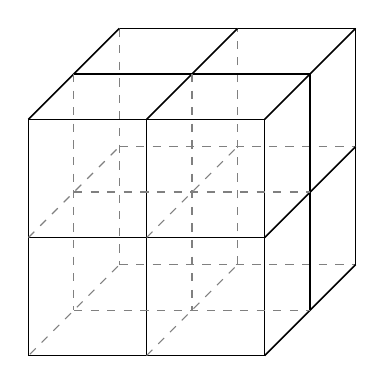
\begin{tikzpicture}[scale = 1]
        %%%%%%%%%%%%%%%%%%%%%%%% Cara trasera %%%%%%%%%%%%%%%%%%%%%%%%%%%%%%%%%%%
        \draw[gray, fill opacity=0.5, dashed] (0,0,0) -- (3,0,0); %Edge inferior punteado
        \draw[line width=0.2mm] (3,0,0) -- (3,3,0); %Edge derecho
        \draw[line width=0.2mm] (3,3,0) -- (0,3,0); %Edge superior
        \draw[gray, fill opacity=0.5, dashed] (0,3,0) -- (0,0,0); %Edge izquierdo punteado
        %%%%%%%%%%%%%%%%%%%%%%%% Cara delantera %%%%%%%%%%%%%%%%%%%%%%%%%%%%%%%%%%
        \draw[line width=0.2mm] (0,0,3) -- (3,0,3); %Edge bajo
        \draw[line width=0.2mm] (3,0,3) -- (3,3,3);
        \draw[line width=0.2mm] (3,3,3) -- (0,3,3);
        \draw[line width=0.2mm] (0,3,3) -- (0,0,3);
        \draw[line width=0.2mm] (0,3,0) -- (0,3,3);
        \draw[line width=0.2mm] (3,3,0) -- (3,3,3);
        \draw[gray, fill opacity=0.5, dashed] (0,0,0.05) -- (0,0,3); %Línea entre caras
        \draw[line width=0.2mm] (3,0,0) -- (3,0,3);
        %%%%%%%%%%%%%%%%%%% Mallado: caras delantera y trasera %%%%%%%%%%%%%%%%%%%%%%%%%%%%%
        \draw[line width=0.2mm] (0,1.5,3) -- (3,1.5,3);
        \draw[line width=0.2mm] (1.5,0,3) -- (1.5,3,3);
        \draw[gray, fill opacity=0.5, dashed] (0,1.5,0) -- (3,1.5,0);
        \draw[gray, fill opacity=0.5, dashed] (1.5,0,0) -- (1.5,3,0);
        %%%%%%%%%%%%%%%%%%%%%% Mallado: caras superior e inferior %%%%%%%%%%%%%%%%%%%%%%%%%%%
        \draw[line width=0.2mm] (0,3,1.5) -- (3,3,1.5);
        \draw[line width=0.2mm] (1.5,3,3) -- (1.5,3,0);
        \draw[gray, fill opacity=0.5, dashed] (0,0,1.5) -- (3,0,1.5);
        \draw[gray, fill opacity=0.5, dashed] (1.5,0,3) -- (1.5,0,0);
        %%%%%%%%%%%%%%%%%%%%%% Mallado: caras laterales %%%%%%%%%%%%%%%%%%%%%%%%%%%%%%%%
        \draw[line width=0.2mm] (3,3,1.5) -- (3,0,1.5);
        \draw[line width=0.2mm] (3,1.5,3) -- (3,1.5,0);
        \draw[gray, fill opacity=0.5, dashed] (0,3,1.5) -- (0,0,1.5);
        \draw[gray, fill opacity=0.5, dashed] (0,1.5,3) -- (0,1.5,0);
        %%%%%%%%%%%%%%%%%%%%%% Mallado: líneas interiores %%%%%%%%%%%%%%%%%%%%%%%%%%%%%%%
        \draw[gray, fill opacity=0.5, dashed] (0,1.5,1.5) -- (3,1.5,1.5);
        \draw[gray, fill opacity=0.5, dashed] (1.5,1.5,3) -- (1.5,1.5,0);
        \draw[gray, fill opacity=0.5, dashed] (1.5,3,1.5) -- (1.5,0,1.5);
        %%%%%%%%%%%%%%%%%%%%%% Algunos nodos %%%%%%%%%%%%%%%%%%%%%%%%%%%%%%%%%%%%
      \end{tikzpicture}
      \caption{Refined $3$D element}
      \label{subfig:ref3Delement}
    \end{center}
  \end{subfigure}
  \caption{Hierarchical isotropic mesh element subdivision for $3$D cases.}
  \label{fig:Hierarchi3D}
\end{figure}

\subsection{Supported refinements and unrefinements}
\label{subsec:SuppRef}
We devote this subsection to illustrate  mesh operations for a given element $K$. We define a node $e$ as a component of an element $K$ such that $e$ is either a vertex, an edge, a face, or a volume. The dimension $d_{e} \in \{0, \cdots, d\}$ of $e$ reads as follows: $d_{e} = 0$ for a vertex, $d_{e} = 1$ denotes an edge, $d_{e} = 2$ stands for a face and $d_{e} = 3$ for a volume. This way, a node $e$ of dimension $d_{e} \neq 0$ has a subset $\calD_{e} \subseteq \{1, \cdots, d\}$ of  $d_{e}$ directions, with $d$ denoting the spatial dimension of the problem.

We define a $p$-(un)refinement of one node $e$ of $K$ in one direction $i$ as follows: a $p$-refinement sets $p$ to $p+\mathds{1}_{i}$ and a $p$-unrefinement sets $p$ to $\textrm{max} (p - \mathds{1}_{i}, 1)$ where $\mathds{1}_{i}$ is a vector of dimension $d$ with $1$ in the $i^{\textrm{th}}$ component and $0$ everywhere else.

When we execute an $h$-refinement, then we create leaf elements (see \Cref{subfig:href}). These leaf elements inherit the orders of $K$. When we execute an $h$-unrefinement (see \Cref{subfig:hunref}), then we trim the tree, and the root element inherits the maximum orders of its leaves. Note that an $h$-unrefinement has no effect over the initial mesh.

\begin{figure}
  \begin{subfigure}[]{0.45\textwidth}
    \begin{center}
      \tikzsetnextfilename{Hier1}
      \begin{tikzpicture}[scale=1]%,every node/.style={minimum size=1cm},on grid]
        \begin{scope}[yshift=0]
          \begin{axis}[view={40}{70}, ticks=none,hide axis,]
            \addplot3[patch, patch type=rectangle,
              patch refines=1, mesh, black, thick,
              z filter/.code={\def\pgfmathresult{-0.0}} % change that number to translate the "mesh" (beware it may change the color mapping)
            ] coordinates {
                (0,0,0) (3,0,0) (3,3,0) (0,3,0)
              };

            \coordinate (a) at (0,0,0);
            \coordinate (b) at (1.5,0,0);
            \coordinate (c) at (1.5,1.5,1);
            \coordinate (d) at (0,1.5,0);


            \addplot3[
              surfBF,
              domain=0:3/2,domain y=3/2:3,
            ]
            {(-4*x*(-3+y))/9};
            \addplot3[
              meshBF,
              domain=0:3/2,domain y=3/2:3,
            ]
            {(-4*x*(-3+y))/9};

            \addplot3[
              surfBF1,
              domain=0:3/2,domain y=0:3/2,
            ]
            {(4*x*y)/9};
            \addplot3[
              meshBF,
              domain=0:3/2,domain y=0:3/2,
            ]
            {(4*x*y)/9};

            \addplot3[
              surfBF,
              domain=3/2:3,domain y=0:3/2,
            ]
            {(-4*(-3+x)*y)/9};
            \addplot3[
              meshBF,
              domain=3/2:3,domain y=0:3/2,
            ]
            {(-4*(-3+x)*y)/9};

            \addplot3[
              surfBF,
              domain=3/2:3,domain y=3/2:3,
            ]
            {(4*(-3+x)*(-3+y))/9};
            \addplot3[
              meshBF,
              domain=3/2:3,domain y=3/2:3,
            ]
            {(4*(-3+x)*(-3+y))/9};

          \end{axis}

        \end{scope}
        \begin{scope}[yshift=100]
          \begin{axis}[view={40}{77}, ticks=none,hide axis,xmax=3,ymax=3]
            % \addplot3[patch, patch type=rectangle,opacity=0,
            % patch refines=1, mesh, black, thick,
            % z filter/.code={\def\pgfmathresult{-0.0}} % change that number to translate the "mesh" (beware it may change the color mapping)
            % ] coordinates {
            % 	(0,0,0) (3,0,0) (3,3,0) (0,3,0)
            % };
            \addplot3[patch, patch type=rectangle,
              patch refines=1, mesh, black, thick,
              z filter/.code={\def\pgfmathresult{-0.0}} % change that number to translate the "mesh" (beware it may change the color mapping)
            ] coordinates {
                (0,0,0) (3/2,0,0) (3/2,3/2,0) (0,3/2,0)
              };

            \coordinate (e) at (0,0,0);
            \coordinate (f) at (3/2,0,0);
            \coordinate (g) at (3/2,3/2,0);
            \coordinate (h) at (0,3/2,-3.5);

            \addplot3[
              surfBF,
              domain=0:3/4,domain y=3/4:3/2,
            ]
            {(-8*x*(-3+2*y))/9};
            \addplot3[
              meshBF,
              domain=0:3/4,domain y=3/4:3/2,
            ]
            {(-8*x*(-3+2*y))/9};

            \addplot3[
              surfBF,
              domain=0:3/4,domain y=0:3/4,
            ]
            {(16*x*y)/9};
            \addplot3[
              meshBF,
              domain=0:3/4,domain y=0:3/4,
            ]
            {(16*x*y)/9};

            \addplot3[
              surfBF,
              domain=3/4:3/2,domain y=0:3/4,
            ]
            {(-8*(-3+2*x)*y)/9};
            \addplot3[
              meshBF,
              domain=3/4:3/2,domain y=0:3/4,
            ]
            {(-8*(-3+2*x)*y)/9};

            \addplot3[
              surfBF,
              domain=3/4:3/2,domain y=3/4:3/2,
            ]
            {(4*(-3+2*x)*(-3+2*y))/9};
            \addplot3[
              meshBF,
              domain=3/4:3/2,domain y=3/4:3/2,
            ]
            {(4*(-3+2*x)*(-3+2*y))/9};


          \end{axis}

        \end{scope}
        \draw[thick,fill opacity=1.1,dashed] (a)--(e);
        \draw[thick,fill opacity=1.1,dashed] (b)--(f);
        \draw[thick,fill opacity=1.1,dashed] (c)--(g);
        \draw[thick,fill opacity=1.1,dashed] (d)--(h);
      \end{tikzpicture}
      \caption{$h$-refinement}
      \label{subfig:href}
    \end{center}
  \end{subfigure}
  \begin{subfigure}[]{0.45\textwidth}
    \begin{center}
      \tikzsetnextfilename{Hier2}
      \begin{tikzpicture}[scale=1]%,every node/.style={minimum size=1cm},on grid]
        \begin{scope}[yshift=0]
          \begin{axis}[view={40}{70}, ticks=none,hide axis,]
            \addplot3[patch, patch type=rectangle,
              patch refines=1, mesh, black, thick,
              z filter/.code={\def\pgfmathresult{-0.0}} % change that number to translate the "mesh" (beware it may change the color mapping)
            ] coordinates {
                (0,0,0) (3,0,0) (3,3,0) (0,3,0)
              };

            \coordinate (a) at (0,0,0);
            \coordinate (b) at (1.5,0,0);
            \coordinate (c) at (1.5,1.5,1);
            \coordinate (d) at (0,1.5,0);


            \addplot3[
              surfBF,
              domain=0:3/2,domain y=3/2:3,
            ]
            {(-4*x*(-3+y))/9};
            \addplot3[
              meshBF,
              domain=0:3/2,domain y=3/2:3,
            ]
            {(-4*x*(-3+y))/9};

            \addplot3[
              surfBF,
              domain=0:3/2,domain y=0:3/2,
            ]
            {(4*x*y)/9};
            \addplot3[
              meshBF,
              domain=0:3/2,domain y=0:3/2,
            ]
            {(4*x*y)/9};

            \addplot3[
              surfBF,
              domain=3/2:3,domain y=0:3/2,
            ]
            {(-4*(-3+x)*y)/9};
            \addplot3[
              meshBF,
              domain=3/2:3,domain y=0:3/2,
            ]
            {(-4*(-3+x)*y)/9};

            \addplot3[
              surfBF,
              domain=3/2:3,domain y=3/2:3,
            ]
            {(4*(-3+x)*(-3+y))/9};
            \addplot3[
              meshBF,
              domain=3/2:3,domain y=3/2:3,
            ]
            {(4*(-3+x)*(-3+y))/9};

          \end{axis}

        \end{scope}
        \begin{scope}[yshift=100]
          \begin{axis}[view={40}{77}, ticks=none,hide axis,xmax=3,ymax=3]
            % \addplot3[patch, patch type=rectangle,opacity=0,
            % patch refines=1, mesh, black, thick,
            % z filter/.code={\def\pgfmathresult{-0.0}} % change that number to translate the "mesh" (beware it may change the color mapping)
            % ] coordinates {
            % 	(0,0,0) (3,0,0) (3,3,0) (0,3,0)
            % };
            \addplot3[patch, patch type=rectangle,
              patch refines=1, mesh, black, thick,
              z filter/.code={\def\pgfmathresult{-0.0}} % change that number to translate the "mesh" (beware it may change the color mapping)
            ] coordinates {
                (0,0,0) (3/2,0,0) (3/2,3/2,0) (0,3/2,0)
              };

            \coordinate (e) at (0,0,0);
            \coordinate (f) at (3/2,0,0);
            \coordinate (g) at (3/2,3/2,0);
            \coordinate (h) at (0,3/2,-3.5);

            \addplot3[
              surfBF1,
              domain=0:3/4,domain y=3/4:3/2,
            ]
            {(-8*x*(-3+2*y))/9};
            \addplot3[
              meshBF,
              domain=0:3/4,domain y=3/4:3/2,
            ]
            {(-8*x*(-3+2*y))/9};

            \addplot3[
              surfBF1,
              domain=0:3/4,domain y=0:3/4,
            ]
            {(16*x*y)/9};
            \addplot3[
              meshBF,
              domain=0:3/4,domain y=0:3/4,
            ]
            {(16*x*y)/9};

            \addplot3[
              surfBF1,
              domain=3/4:3/2,domain y=0:3/4,
            ]
            {(-8*(-3+2*x)*y)/9};
            \addplot3[
              meshBF,
              domain=3/4:3/2,domain y=0:3/4,
            ]
            {(-8*(-3+2*x)*y)/9};

            \addplot3[
              surfBF1,
              domain=3/4:3/2,domain y=3/4:3/2,
            ]
            {(4*(-3+2*x)*(-3+2*y))/9};
            \addplot3[
              meshBF,
              domain=3/4:3/2,domain y=3/4:3/2,
            ]
            {(4*(-3+2*x)*(-3+2*y))/9};


          \end{axis}

        \end{scope}
        \draw[thick,fill opacity=1.1,dashed] (a)--(e);
        \draw[thick,fill opacity=1.1,dashed] (b)--(f);
        \draw[thick,fill opacity=1.1,dashed] (c)--(g);
        \draw[thick,fill opacity=1.1,dashed] (d)--(h);
      \end{tikzpicture}
      \caption{$h$-unrefinement}
      \label{subfig:hunref}
    \end{center}
  \end{subfigure}
  \caption{Mesh operations for a given leaf element $K$. In both cases, the final mesh is made up of colored elements. }
  \label{Fig:Mesh}
\end{figure}

\subsection{Removable basis functions}
\label{subsec:Removable}
Based on Darrigrand's \emph{removable} basis functions definition \cite{darrigrand2020painless}, we recall that \emph{removable} basis functions are those that can be directly removed from the discretization without affecting the others. Let us simply denote the set of removable basis functions of an element $K \in \calT$ as $R_{\textrm{m}}(K)$, and its cardinality as $|R_{\textrm{m}}(K)|$.
When identified, they will be removed in the unrefinement iterative process. For instance, in \Cref{fig:linearremovable}, the product of linear shape functions (in grey) is removable. For details about defining \emph{removable} basis functions, we refer the reader to \cite{darrigrand2020painless}.
%Note to myself:  $P_{4}^{x} P_{4}^{y}$ in the same plane as their drawings.

\begin{figure}

  \newsavebox\foobox
  \newcommand\slbox[2]{%
    \FPdiv{\result}{#1}{57.296}% CONVERT deg TO rad
    \FPtan{\result}{\result}%
    \slantbox[\result]{#2}%
  }%
  \newcommand{\slantbox}[2][30]{%
    \scalebox{1}[.7]{\mbox{%
        \sbox{\foobox}{#2}%
        \hskip\wd\foobox
        \pdfsave
        \pdfsetmatrix{1 0 #1 1}%
        \llap{\usebox{\foobox}}%
        \pdfrestore
      }}}
  \newcommand\rotslant[3]{\rotatebox{#1}{\slbox{#2}{#3}}}

  \usetikzlibrary{positioning,patterns,shapes}
  \usepgfplotslibrary{external}
  \usetikzlibrary{decorations.markings,intersections,calc}
  \usetikzlibrary{decorations.pathreplacing}
  \usetikzlibrary{fpu}

  \usepgfplotslibrary{colormaps}
  \usepgfplotslibrary{colorbrewer}
  \usepgfplotslibrary{patchplots}

  \pgfplotsset{compat=newest}


  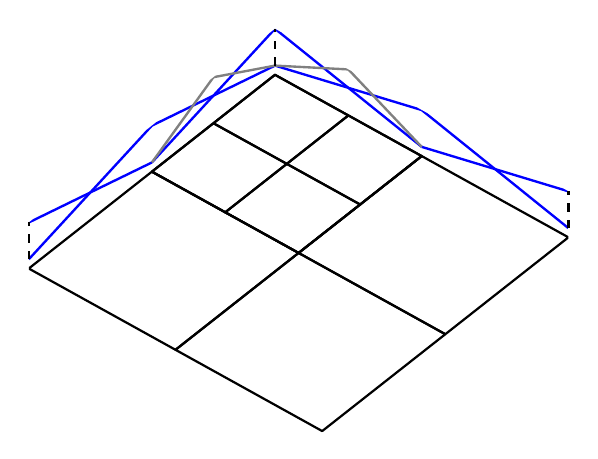
\begin{tikzpicture}[scale=1]%,every node/.style={minimum size=1cm},on grid]
    \begin{axis}[view={40}{70}, ticks=none,hide axis,]
      \addplot3[patch, patch type=rectangle,
        patch refines=1, mesh, black, thick,
        z filter/.code={\def\pgfmathresult{-0.0}} % change that number to translate the "mesh" (beware it may change the color mapping)
      ] coordinates {
          (0,0,0) (10,0,0) (10,10,0) (0,10,0)
        };

      \addplot3[patch, patch type=rectangle,
        patch refines=1, mesh, black, thick,
        z filter/.code={\def\pgfmathresult{-0.0}} % change that number to translate the "mesh" (beware it may change the color mapping)
      ] coordinates {
          (0,5,0) (0,10,0) (5,10,0) (5,5,0)
        };


      \coordinate (a) at (0,0,0.2);
      \coordinate (b) at (0,0,1);

      \coordinate (i) at (10,10,0.2);
      \coordinate (j) at (10,10,1);

      \coordinate (k) at (0,10,0.2);
      \coordinate (l) at (0,10,1);

      \draw[blue,line width=0.3mm] (0,10,0.2) -- (5,10,1);
      \draw[blue,line width=0.3mm] (5,10,1) -- (10,10,0.2);

      \draw[blue,line width=0.3mm] (0,10,1) -- (5,10,0.2);
      \draw[blue,line width=0.3mm] (5,10,0.2) -- (10,10,1);

      \draw[gray,line width=0.3mm] (0,10,0.2) -- (2.5,10,1);
      \draw[gray,line width=0.3mm] (2.5,10,1) -- (5,10,0.2);

      \draw[blue,line width=0.3mm] (0,0,0.2) -- (0,5,1);
      \draw[blue,line width=0.3mm] (0,5,1) -- (0,10,0.2);

      \draw[blue,line width=0.3mm] (0,0,1) -- (0,5,0.2);
      \draw[blue,line width=0.3mm] (0,5,0.2) -- (0,10,1);

      \draw[gray,line width=0.3mm] (0,5,0.2) -- (0,7.5,1);
      \draw[gray,line width=0.3mm] (0,7.5,1) -- (0,10,0.2);

    \end{axis}
    \draw[thick,fill opacity=1,dashed] (a)--(b);
    \draw[thick,fill opacity=1,dashed] (i)--(j);
    \draw[thick,fill opacity=1,dashed] (k)--(l);
  \end{tikzpicture}
  \caption{Removable linear shape functions (grey).}
  \label{fig:linearremovable}
\end{figure}
